% Copyright (c) 2020 Carl Martin Ludvig Sinander.

% This program is free software: you can redistribute it and/or modify
% it under the terms of the GNU General Public License as published by
% the Free Software Foundation, either version 3 of the License, or
% (at your option) any later version.

% This program is distributed in the hope that it will be useful,
% but WITHOUT ANY WARRANTY; without even the implied warranty of
% MERCHANTABILITY or FITNESS FOR A PARTICULAR PURPOSE. See the
% GNU General Public License for more details.

% You should have received a copy of the GNU General Public License
% along with this program. If not, see <https://www.gnu.org/licenses/>.

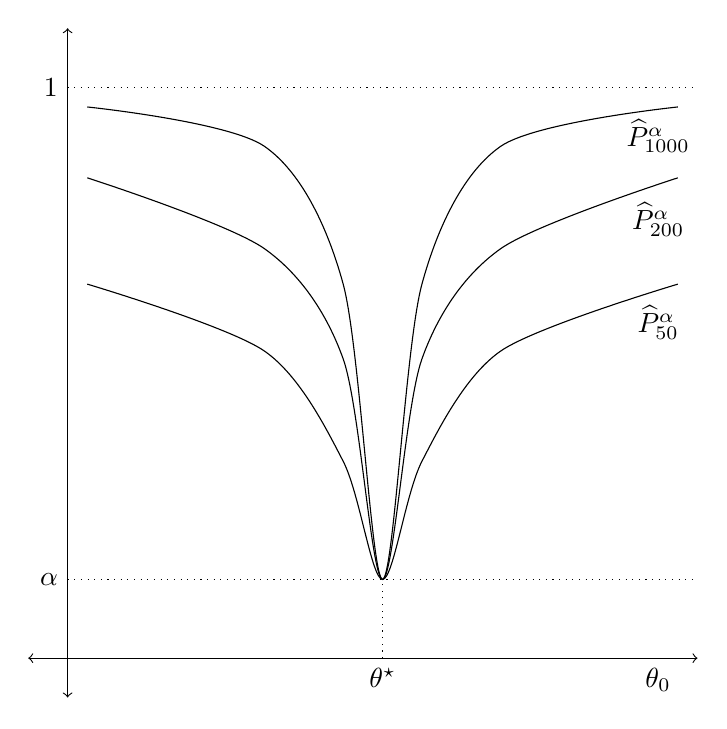
\begin{tikzpicture}[scale=1]
	
	% power envelopes
	\draw plot [smooth] coordinates {
	(0.25,7) 
	(2.5,6.5) 
	(3.5,4.75) 
	(4,1) 
	(4.5,4.75) 
	(5.5,6.5) 
	(7.75,7)};
	\draw plot [smooth] coordinates {
	(0.25,7*0.8+0.5) 
	(2.5,6.5*0.8) 
	(3.5,4.75*0.8) 
	(4,1) 
	(4.5,4.75*0.8) 
	(5.5,6.5*0.8) 
	(7.75,7*0.8+0.5)};
	\draw plot [smooth] coordinates {
	(0.25,7*0.6+0.55) 
	(2.5,6.5*0.6) 
	(3.5,4.75*0.6-0.35) 
	(4,1) 
	(4.5,4.75*0.6-0.35) 
	(5.5,6.5*0.6) 
	(7.75,7*0.6+0.55)};

	% power envelope labels
	\draw (7.5,6.97) node[anchor=north] {$\widehat{P}^\alpha_{1000}$};
	\draw (7.5,5.91) node[anchor=north] {$\widehat{P}^\alpha_{200}$};
	\draw (7.5,4.6) node[anchor=north] {$\widehat{P}^\alpha_{50}$};

	% axis labels
	%\draw (0,4.5) node[anchor=south,rotate=90] {$\text{rejection probability}$};	
	\draw (7.5,0) node[anchor=north] {$\theta_0$};

	% null
	\draw (4,0) node[anchor=north] {$\theta^\star$};	
	\draw[-,dotted] (4,0)--(4,1);
	%\draw[-] (4,-0.125)--(4,0.125);

	% size
	\draw (0,1) node[anchor=east] {$\alpha$};	
	\draw[-,dotted] (0,1)--(8,1);

	% probability 1
	\draw (0,7.25) node[anchor=east] {$1$};	
	\draw[-,dotted] (0,7.25)--(8,7.25);


	% axes
	\draw[<->] (-0.5,0) -- (8,0);
	\draw[<->] (0,-0.5) -- (0,8);
	%\fill (-0.007,-0.007) rectangle (0.007,0.007);

\end{tikzpicture}